%\documentclass[lineno]{jfm}
\documentclass[lineno]{JFM-FLM_Au}
\usepackage[percent]{overpic}
\usepackage{float}
\usepackage{import}
\usepackage{transparent}
\usepackage{natbib}

%\usepackage{showframe}

\newtheorem{lemma}{Lemma}
\newtheorem{corollary}{Corollary}

\lefttitle{G.A. Kerr, and L. Kreplak}
\righttitle{Journal of Fluid Mechanics}

\title{Liquid Bridge Stabilization by Surface Skin Formation Enables Contact Drawing of Protein Microfibres}

\author{
	Gavin A. Kerr\aff{1}, 
	Grace O'Connor\aff{1},
	Grecia Valeria Sanchez Ruiz\aff{1},
	Hessam Yaghoobi Koopaee\aff{1},
	\and Laurent Kreplak\aff{1}
}
\affiliation{
	\aff{1}Dalhousie University, Department of Physics and Atmospheric Science, 6385 South St, Halifax, NS B3H 4J4, Canada
}

\corresau{Laurent Kreplak, \email{kreplak@dal.ca}}

\begin{document}
\maketitle

\begin{abstract}
The thinning dynamics of a liquid bridge is well-understood in the limit where surface tension and capillary forces dominate. As the viscosity of the fluid increases, liquid bridges become increasingly stable with break up times in the order of seconds. In the case of entangled polymer solutions, this property can be leveraged to draw up to one-meter-long bridges with diameters in the micron range that survive long enough to dry into microfibres. The accepted explanation for the survival of the bridge is that elastic forces within the entangled polymer solution resist capillary induced thinning. Here we explore an alternative explanation by attempting to draw microfibres from a concentrated protein solution. We show that the maize storage protein zein which is soluble in ethanol/water mixtures behaves as a thixotropic elastoviscoplastic (TEVP) fluid at concentrations above 50\% by weight and can be drawn into 10 cm long microfibres.  However robust microfibre formation occurs over a narrow window of viscosity due to capillary induced failures at low viscosity and elastic-like failure at high viscosity. Videomicroscopy reveals that the elastic failure mode is due to the rupture of a TEVP skin at the surface of the bridge. To further demonstrate the generality of this skin formation mechanism for liquid bridge stabilization, we form microfibres using an 80\% by weight solution of short collagen peptides, 2-5 kDa, dissolved in pure water. Overall, our findings are opening the road for the green manufacturing of protein microfibres without the need for harsh volatile solvents.
\end{abstract}

%{\bf MSC Codes }  {\it(Optional)} Please enter your MSC Codes here


\section{Introduction}

Liquid bridges were initially described by Thomas Young in 1804 \cite{thomas_iii_1804} and are formed when two surfaces are brought close together and a liquid fills the gap between them. By increasing the distance between the surfaces, the liquid bridge becomes elongated. Depending on the properties of the fluid, the time scale over which the liquid remains stable (does not rupture) can vary significantly. For low viscosity liquids like water, the bridge is dominated by capillary forces which act to minimize the surface area. Within this limit, the shape of a static liquid bridge is determined by the Young-Laplace equation \cite{meseguer_review_1995}. When separating the two surfaces, the capillary forces will thin and rupture the bridge on the order of a fraction of a second or less \cite{coriell_stability_1977}. There are classes of liquids such as polymer solutions which can form stable liquid bridges over much longer time scales. For example, methyl-cellulose solutions can form liquid bridges which remain stable for up to 10 seconds \cite{morozova_extensional_2018}. Depending on the concentration of methyl-cellulose, the solutions have viscosities in the range of 1-100 Pa$\cdot$s and are viscoelastic due to chain entanglement \cite{morozova_extensional_2018}. The thinning dynamics of the liquid bridges of entangled polymer solutions is well understood by breaking the process into regimes where different forces dominate \cite{dinic_macromolecular_2019}. The initial regime is driven by inertiocapillary or viscocapillary forces, depending on the viscosity of the solution, and is characterized by the liquid bridge diameter thinning according to a power law. The second regime is dominated by elastocapillary forces due to stretching of the entangled polymer chains. This regime is characterized by an exponential decay in the diameter of the bridge. It can be used to measure properties of the solution such as the extensional relaxation time and its elastic storage modulus. Then finally there is a terminal regime due to the finite extensibility of the polymer chains. This regime is characterized by a rapid decrease in the diameter of the liquid bridge which leads to rupture.

The process of creating long-lasting liquid bridges from viscous polymer solutions has been leveraged as a technique for fiber fabrication. This method has existed under various names, such as hand drawing \cite{cho_synthesis_2011}, however it has more recently been studied under the name \emph{contact drawing} by Frampton et al.~\cite{frampton_elongation_2015}. Unlike traditional methods that suspend a droplet between two surfaces, contact drawing forms a liquid bridge between a pin and a solution reservoir. The pin penetrates the reservoir and then accelerates outward. After traveling a set distance, the pin stops. Under appropriate solution properties and drawing conditions, the liquid bridge remains stable between the pin and the reservoir and dries to form a fiber \cite{chowdhry_polymer_2021}. These fibers can be collected and used in various applications \cite{verma_multi-pin_2022}. By analyzing the time scale over which the liquid bridge remains stable before rupture, the reptation time $t_{\text{rep}}$ can be estimated. This is the characteristic time scale over which the polymer chains become disentangled \cite{colby_structure_2010}. The key principle is that the drawing time must be less than $t_{\text{rep}}$ to elicit an elastic rather than a viscous response, which can resist capillary thinning to stabilize the fiber \cite{chowdhry_polymer_2021}. Reptation theory predicts $t_{\text{rep}} \sim M_w^3$ \cite{colby_structure_2010}, and empirically, an exponential relationship between polymer concentration (\% weight) and $t_{\text{rep}} / M_w^3$ has been demonstrated \cite{chowdhry_polymer_2021}. This was validated using viscous dextran solutions ($\sim$10 Pa$\cdot$s) with molecular weights ranging from 70 to 500 kDa. According to this measured exponential relationship, 70 kDa Dextran at a concentration around $60\%$ by weight has a predicted $t_{\text{rep}}$ of 1 second and decreasing the concentration by only $15\%$ leads to a 500 fold decrease in $t_{\text{rep}}$. While fiber formation at high molecular weights and lower concentration has been experimentally demonstrated using polyethylene oxide (PEO), attempts at lower molecular weights and higher concentrations remain limited due to the exceedingly high draw velocities required, 100~m/s or more, surpassing the capabilities of typical contact drawing systems, which operate at velocities less than 1~m/s \cite{chowdhry_polymer_2021,verma_multi-pin_2022}. Within these experimental limits, contact drawn fibers typically range from 0.1 to 10 microns in diameter, depending on the solution composition. Fiber lengths are typically on the order of 0.1 to 1 m. The method can be scaled for bulk fiber production by employing arrays of pins \cite{verma_multi-pin_2022}, and has been demonstrated for various polymer solutions, including dextran \cite{chowdhry_polymer_2021}, polyethylene oxide (PEO) \cite{yaghoobi_multifilament_2023}, and polyvinyl alcohol \cite{visser_loading_2022}. To date, contact drawing has only been applied to polymer solutions. However, these polymer solutions can be combined with other materials for diverse applications. For example, PEO has been combined with collagen \cite{yaghoobi_multifilament_2023} and fibrin \cite{verma_nonwoven_2023} to produce fibers for tissue engineering applications. To expand the application of contact drawing, it would be beneficial to find protein solutions that can be drawn into fibers without the need for a polymer. Encouragingly, one natural example is silk which is produced by spiders and silkworms using a pultrusion process \cite{sparkes_analysis_2017} akin to contact drawing without a pin \cite{ni_biomimetic_2022}.

One potential candidate protein is alpha zein, the maize storage protein, which is mostly $\alpha$-helical \cite{argos_structural_1982} and forms micelles like some silk proteins in ethanol water mixtures \cite{parent_hierarchical_2018,uzun_characterization_2017}. zein solutions can be processed into fibers using various techniques, including wet spinning \cite{cui_development_2022}, electrospinning \cite{rahman_fabrication_2023} and centrifugal spinning \cite{brum_facile_2025} which shares some similarities with contact drawing, i.e. it is a dry spinning process relying on the formation of a liquid jet. 
Although zein is a promising candidate for contact-drawing, its molecular weight of 22 kDa would require preparing a solution at a concentration well above the maximum solubility of zein in binary solvents ($60\%$ w/w \cite{shukla_zein_2001}) to successfully draw a 0.1 m long fiber.
This estimate assumes zein behaves like an entangled polymer solution, and that the $t_{\text{rep}}$ dependency with molecular weight described above \cite{chowdhry_polymer_2021} also applies. 
In this study, we show that zein dissolved in ethanol-water mixtures can in fact be processed into fibers by contact drawing at around $50\%$ by weight due to the formation of a solid-like skin layer at the liquid air interface that stabilizes the liquid bridge against capillary thinning. The presence of the skin gives rise to an elastic failure mode and leads to a narrow window of concentrations over which contact drawing can occur with a $100\%$ success rate. These findings extend the use of contact drawing beyond polymer solutions and point to skin formation as a mechanism to stabilize a liquid bridge over long time scales, as recently hypothesized by Colby \cite{colby_fiber_2023}. 

\section{Experimental Methods}
\paragraph*{Materials and Solution Preparation}
zein powder from Sigma-Aldrich, with a molecular weight of 22 kDa, was used to prepare ethanol-water protein solutions one day prior to experimentation. Solutions were prepared by gradually adding zein to ethanol-water mixtures ($70$-$90$\% v/v ethanol in water) while stirring. The zein concentration ranged from 41\% to 57\% by total weight. Solutions were stored at $4^\circ$C for 24 hours, then stirred again to ensure all the zein was fully dissolved. Next, solutions were centrifuged at 4500 RCF for 20 minutes at $4^\circ$C to remove any air bubbles introduced into the solution by stirring. Finally, the solutions were left out for approximately 20 minutes before use to allow them to reach room temperature (22$^\circ$C). Collagen I peptides enzymatically extracted from Atlantic Cod fish skin was purchased from 3F Waste Recovery (Newfoundland, Canada). The peptides were provided as a freeze dried powder and a molecular weight between 2 and 5 kDa. The peptides were dissolved in pure water while stirring and stored at $4^\circ$C until use.

\paragraph*{Rheology}
Solution viscosities were characterized using a TA HR10 Rheometer with a parallel plate geometry. A 1 mm gap was used for all measurements. Silicone oil was applied to the edges of the solution between the plates to prevent evaporation during measurements. The temperature was constant at 22$^\circ$C. For zein solutions, viscosity data were obtained from flow sweep tests, where a series of constant shear rates are applied and the resulting shear stresses are recorded. For cod collagen solutions, small amplitude oscillatory shear tests were used. For each sample, the range of shear rates was $0.01$ to $100$ s$^{-1}$ with 5 points per decade. The zero shear viscosity $\eta_0$ was calculated by fitting the measured viscosity as a function of shear rate to the Cross model $\eta(\dot{\gamma}) = \eta_{\infty} + \dfrac{\eta_0 - \eta_{\infty}}{1 + (K\dot{\gamma})^m}$ where $\eta_\infty$ is the infinite shear viscosity, $K$ is the cross constant (indicative of the onset shear thinning), and $m$ is the shear thinning index \cite{barnes_handbook_2000}. Fitting was achieved using non-linear least squares optimization and implemented with the \texttt{curve\_fit} function from the \texttt{scipy.optimize} module in Python. Additionally, peak hold tests were performed on a few zein solutions. The solutions were held at a constant shear rate between 1-100 s$^{-1}$ for 300 seconds while monitoring the apparent viscosity.

\paragraph*{Contact Drawing Procedure}
Contact drawing was performed using a custom-built platform consisting of a belt-driven car with an attached cylindrical pin (diameter: 600 $\mu$m), which was used to draw a liquid bridge from a solution reservoir. The liquid bridge was illuminated from below by a light source and diffuser, allowing the bridge silhouette to be captured by an overhead camera (Basler ace2 a2A1920-160umBAS Monochrome) with a frame rate of 135 fps mounted on a stereomicroscope with a magnification of 1.5x. The zein or cod collagen peptide solutions were top-loaded into a trough-shaped reservoir (length: 18 mm, width: 4 mm, height: 6 mm) that was open at one end. High solution viscosity allowed the solution to remain in the reservoir. A spatula was used to create a flat interface at the entry point of the pin. Within two seconds of preparing the solution reservoir, the drawing process was initiated. The pin entered the reservoir, paused for 0.5 seconds, then was drawn away from the reservoir at a constant acceleration of 1000 mm/s$^2$ until a maximum draw velocity of up to 300 mm/s was reached over a distance of 100 mm. The camera continued to capture images for up to two additional seconds post-drawing depending on the draw velocity. For each solution condition and/or draw velocity, this procedure was repeated between 10 and 30 times at a relative humidity between 20 and 30\%RH. 
 
Custom software was developed in Rust to analyze images captured during the fiber drawing process. The software measures the fiber diameter at the edge of the image, which is 3 mm from the solution reservoir. This is achieved by first applying a small Gaussian blur to reduce noise, followed by a threshold filter to isolate the fiber from the background. The number of non-zero pixels along the specified edge is then counted and converted to physical units using a calibrated pixel-to-length scaling factor determined from the known pin diameter in frame. In addition, each image sequence is manually labeled to identify the rupture frame and classify the failure mode.
 
\paragraph*{Scanning Electron Microscopy}
Collagen I peptide fibers were contact drawn from an 80\% by weight solution in water using a custom-designed pin array and a flat paddle as described in \cite{yaghoobi_multifilament_2023}. Fibers were laid down on carbon tape, a 5 nm gold/palladium (80/20) layer was applied with a sputter coater EM ACE600 (Leica Microsystems) and imaged at an accelerating voltage of 5 kV using a Sigma 300 VP Field Emission SEM (Zeiss).

\section{Results and Discussion}
\paragraph*{Thixotropic behaviour of concentrated zein solutions}
The zero shear viscosity results from the cross model fits are shown in figure \ref{fig:flow_sweep_example}A and B, for zein, collagen peptides and dextran \cite{chowdhry_polymer_2021} solutions. The viscosity of the zein solutions increases exponentially with zein concentration. Solutions with 70\% and 80\% ethanol follow similar trends, whereas 90\% ethanol solutions exhibit a significantly higher viscosity at lower concentrations. Although the slopes are similar, less zein is required to achieve the same viscosity in 90\% ethanol. This is consistent with a previous study describing structural transitions of zein micelles with increasing ethanol concentration \cite{kim_aggregate_2008}. Even so flow sweep tests indicated mostly Newtonian behaviour, we used peak hold tests to explore Non-Newtonian character for two different zein concentrations (48\% and 52\% w/w) in 80\% ethanol. The peak hold tests indicate that for lower zein concentrations (48\% w/w) the viscosity remains constant, typical of a Newtonian liquid, over a period of 300 seconds, for shear rates of 1 - 100 s$^{-1}$ (figure \ref{fig:flow_sweep_example}C). For the higher zein concentration (52\% w/w), the behaviour was identical for lower shear rates, however, at the highest shear rate (100 s$^{-1}$) the viscosity decreased from 10 to 0.6 Pa$\cdot$s over a time scale of 100 seconds. After 100 seconds, the viscosity began to increase again (figure \ref{fig:flow_sweep_example}D). This is characteristic of a thixotropic liquid, with shear-induced structural breakdown followed by time-dependent recovery of viscosity \cite{larson_review_2019}. The extensional strain rates experienced by contact drawn zein solutions reach up to 50 s$^{-1}$ but only during a fraction of a second (see Dynamic Cone Diameter Analysis section), so probably not long enough to exhibit the thixotropic behaviour as observed in figure \ref{fig:flow_sweep_example}C. However, during the drawing process, zein solution at the liquid bridge surface is expected to exhibit an increase in viscosity due to the local increase in zein concentration resulting from solvent evaporation. In that scenario, the thixotropic response observed at the highest shear rate may influence the stability of a contact drawn zein liquid bridge and the formation of a zein fiber.

\begin{figure}[tbp]
  \centering
  \def\svgwidth{0.6\textwidth} % or 0.48\textwidth for half-width
  \import{figures/panels/}{viscosity_figure.pdf_tex}
	\caption{
		(A) Zero-shear viscosity measurements of zein solutions in 70\%, 80\%, and 90\% ethanol along with data for 500 kDa dextran in water adapted from \cite{chowdhry_polymer_2021}.
		Each condition is fit with an exponential function.
		The length of the fit line indicates the range of zein concentrations used in this study.
		(B) Zero-shear viscosity for dextran (adapted from Chowdhry et al. \cite{chowdhry_polymer_2021}) and cod collagen peptides in water.
		(C) and (D) Peak hold tests for 48\% and 52\% zein in 80\% ethanol, respectively, corresponding to the labeled points in panel (A).
	}
	\label{fig:flow_sweep_example}
\end{figure}


\subsection{Failure modes of zein liquid bridges}
To visualize the dynamics of fiber formation, the evolution of the liquid bridge was captured using videomicroscopy. These image sequences provide insight into the mechanism by which the fiber breaks or stabilizes during the drawing process. A trial is classified as a success if the bridge forms a continuous fiber that remains intact long after the drawing finishes (such as in figure \ref{fig:failure_mode_sequences}A). Approximately 20 seconds is given to confirm that the fiber remains stable after the drawing is complete. If the bridge breaks, the trial is classified as a failure. Two distinct failure modes are observed, which we have labeled as capillary failures and elastic or solid-like failures. For capillary failures, the bridge thins continuously to a small diameter and breaks at the fluid reservoir (figure \ref{fig:failure_mode_sequences}B). This mode is very similar to the thinning mechanism described by Dinic and Sharma for dilute polymer solutions \cite{dinic_macromolecular_2019}. For elastic failures, the bridge breaks partway along its length, often with visible recoil (figure \ref{fig:failure_mode_sequences}C). This is similar to the failure of a thixotropic elastoviscoplastic (TEVP) liquid bridge under extensional flow (see figure 2 in \cite{chan_edge_2023}) and is consistent with the thixotropic behaviour in shear flow observed at high zein concentration (figure \ref{fig:flow_sweep_example}C). Next, we investigated the prevalence of each failure mode as a function of the solutions' zein concentration and ethanol content.


\begin{figure}[tbp]
  \centering
  \def\svgwidth{0.9\textwidth} % or 0.48\textwidth for half-width
  \import{figures/panels/}{failure_mode_images.pdf_tex}
\caption{
	Representative image sequences showing three failure modes in zein liquid bridge drawing. 
	(A) \emph{Success}: the bridge remains intact and dries into a fiber (49\% zein, 80\% EtOH). 
	(B) \emph{Capillary failure}: the bridge pinches off near the fluid reservoir (47\% zein, 70\% EtOH). 
	(C) \emph{Elastic failure}: the bridge breaks with recoil mid-span (44\% zein, 90\% EtOH). 
	All trials were performed with 1000 mm/s$^2$ acceleration up to a maximum velocity of 200 mm/s (or 10 mm/s for C) over 100 mm. Time stamps indicate time since the start of the drawing process. Scale bars are 500\,$\mu$m.
}
\label{fig:failure_mode_sequences}
\end{figure}


\subsection{High viscosity leads to the elastic failure of zein liquid bridges}
For each ethanol concentration, the fraction of success, capillary failure, and elastic failure is plotted as a function of solution viscosity in figure~\ref{fig:failure_modes}A, C, and E. As expected, low-viscosity zein solutions (below 5~Pa$\cdot$s) are dominated by capillary failures due to rapid thinning and breakup. At high viscosities (above 30~Pa$\cdot$s), elastic failures dominate, likely due to an increase in the TEVP character of the zein solutions. The cumulative distributions of each failure mode are captured by mirrored sigmoid functions, which are collectively minimized in an intermediate viscosity regime. This corresponds to an optimal viscosity window for fiber formation, which is consistently between 7 and 9~Pa$\cdot$s for all three ethanol concentrations tested.

The sigmoid fit parameters (equation \ref{eq:sigmoid_c} and \ref{eq:sigmoid_e}) for each failure type are included in table~\ref{tab:fit_parameters}. For capillary failures, the midpoint viscosity $\eta_C$ decreases from 4.8~Pa$\cdot$s at 70\% ethanol to 2.8~Pa$\cdot$s at 90\% ethanol, indicating that capillary failure occurs at lower viscosities as ethanol content increases. Additionally, the slope $m_C$ decreases from 7.1 to 0.51, indicating a broadening of the capillary failure transition with higher ethanol concentrations.
Elastic failure midpoints $\eta_E$ also shift to lower viscosities with increasing ethanol content, from 35~Pa$\cdot$s at 70\% ethanol to 11~Pa$\cdot$s at 90\%. The slope $m_E$ increases from 0.064 to 0.20, indicating a sharper transition into elastic failure as ethanol concentration increases. This suggests a sharper transition from Newtonian to TEVP character of the zein solutions as the ethanol content increases.

\begin{subequations}\label{eq:sigmoids}
  \begin{equation}
	  f_C(x) = \frac{1}{1 + e^{m_C(\eta_0 - \eta_C)}},
	  \label{eq:sigmoid_c}
  \end{equation}
  \begin{equation}
	f_E(x) = \frac{1}{1 + e^{-m_E(\eta_0 - \eta_E)}}
	\label{eq:sigmoid_e}
  \end{equation}
\end{subequations}

Overall, this means that the effective window for successful fiber formation, given by the difference $|\eta_E - \eta_C|$, narrows with increasing ethanol concentration. At 70\% ethanol, the range is 30.2~Pa$\cdot$s, whereas at 80\% and 90\% ethanol it contracts to 8.7 and 8.2~Pa$\cdot$s, respectively. Thus, while higher ethanol content leads to stronger TEVP character and shifts both failure modes mid-points to lower viscosities, it also reduces the range of viscosities under which stable fiber formation occurs. This window of successful fiber formation is in contrast with the 500kDa dextran data shown in panel (G) of figure~\ref{fig:failure_modes}, which was adapted from Chowdhry et al. \cite{chowdhry_polymer_2021}. In this case, only capillary failures are observed. Given a solution viscosity above a certain threshold (16~Pa$\cdot$s), the solution will form fibers with a 100\% success rate. The lack of elastic failure for dextran liquid bridges is likely due to the extensibility of the entangled polymer network.


\begin{figure}[tbp]
  \centering
  \def\svgwidth{0.8\textwidth} % or 0.48\textwidth for half-width
  \import{figures/panels/}{failure_mode_distribution_95CI.pdf_tex}
	\caption{
		Failure mode distributions at three ethanol concentrations: 70\% (A,B), 80\% (C,D), and 90\% (E,F). 
		Error bars represent 95\% confidence intervals calculated using bootstrap resampling.
		Panels (A), (C), and (E): fraction of successful, capillary, and elastic failures as a function of solution viscosity, with sigmoid fits. 
		Panels (B), (D), and (F): corresponding failure mode fractions as a function of draw velocity at fixed zein concentrations (49\% for 70\% and 80\% ethanol, 44\% for 90\% ethanol). 
		Concentrations were chosen near the peak success rate observed for each solvent condition.
		Panels (G) and (H): failure mode distributions for 500kDa dextran solutions (adapted from \cite{chowdhry_polymer_2021})
	}
	\label{fig:failure_modes}
\end{figure}


\begin{table}
  \begin{center}
\def~{\hphantom{0}}
  \begin{tabular}{lccccc cc}
    Solution
    & \multicolumn{5}{c}{Viscosity (Sigmoid)}
    & \multicolumn{2}{c}{Velocity (Weibull)} \\[3pt]

    & $m_C$ & $\eta_C$
    & $m_E$ & $\eta_E$
    & $|\eta_E-\eta_C|$
    & $k$ & $v'$ \\[3pt]

    Z--$70\%$
    & 7.1  & ~~4.8
    & 0.064 & ~~35
    & ~~30
    & 1.2  & 0.047 \\

    Z--$80\%$
    & 4.4  & ~~4.3
    & 0.32 & ~~13
    & ~~8.7
    & 0.96 & 0.049 \\

    Z--$90\%$
    & 0.51 & ~~2.8
    & 0.20 & ~~11
    & ~~8.2
    & 0.69 & 0.11 \\

    D
    & 0.55 & ~16
    & --   & --
    & --
    & 8.9  & 0.37 \\
  \end{tabular}

  \caption{
  Fit parameters for sigmoid and Weibull functions describing the relationship
  between failure-mode frequency and viscosity or draw velocity
  (see Eq.~\ref{eq:sigmoid_c} and \ref{eq:sigmoid_e} for sigmoid;
  Eq.~\ref{eq:weibull} for Weibull).
  $Z$--70\%, $Z$--80\%, and $Z$--90\% correspond to zein solutions in 70\%, 80\%,
  and 90\% ethanol.
  $D$ corresponds to 500\,kDa dextran in water.
  }
  \label{tab:fit_parameters}
  \end{center}
\end{table}

Failure mode distributions as a function of draw velocity (figure~\ref{fig:failure_modes}B, D, F) measured in the middle of the high-success rate window for each ethanol content reveal two consistent trends. First, success rates increase with velocity. This relationship is captured by a Weibull cumulative distribution function (equation \ref{eq:weibull}) which is a common model for describing probability of failure as a function of time, however, in this case we use draw velocity. This yields both the transition midpoint, $v'$, and the shape parameter, $k$, which quantifies the steepness of the transition.
Second, across the tested range of draw velocities, only elastic failures are observed, suggesting that some amount of TEVP character is required for the zein liquid bridges to survive long enough to dry into fibers. This is especially clear in the 80\% ethanol condition (figure~\ref{fig:failure_modes}D), where a notable decrease in elastic failure frequency, around 48-49\% zein concentration, aligns with the peak for successful trials. Yet at 48\% zein in 80\% ethanol, the peak hold test showed no evidence of TEVP character for all shear rates (figure \ref{fig:flow_sweep_example}B). 
This suggests that TEVP behaviour may arise primarily at the liquid-air interface due to solvent evaporation, rather than in the bulk solution.

\begin{equation}
	f_S(v) = 1 - e^{-(v/v')^k}
	\label{eq:weibull}
\end{equation}

Further insight into the mechanism stabilizing zein liquid bridges can be obtained by comparing to a well-understood polymer system such as dextran in water. For dextran, the transition from failure to success as a function of draw velocity is sharp: Weibull fitting yields a steep shape parameter of $k = 8.9$ and a midpoint scale parameter $v' = 0.37$~m/s, indicating a narrow transition between low and high success rates. Therefore, dextran solutions have a well-defined threshold velocity (over a fixed length of 10 cm) for fiber formation, beyond which success is highly probable. This provides both an accurate criterion for determining fiber formation, and insight into the entanglement mechanism of polymer fiber formation, where the polymer chains must be sufficiently entangled to withstand the stresses of drawing \cite{chowdhry_polymer_2021}. In contrast, zein solutions exhibit broader transitions. Weibull fits for the 70\%, 80\%, and 90\% ethanol conditions yield lower $k$ values of 1.2, 0.97, and 0.69, with corresponding $v'$ values of 0.047, 0.049, and 0.11~m/s. These lower shape parameters indicate that there is a more gradual increase in success rate with draw velocity for zein solutions. As a result, draw velocity is not a reliable predictor of fiber formation for zein solutions near $v'$. This lack of a well-defined time scale for zein fiber formation by contact drawing and the fact that structural recovery of a bulk zein solution showing TEVP character takes 100 seconds in the bulk points again to some kind of surface effect. Colby recently proposed that in polymer solutions, long-lasting liquid bridges are not stabilized by chain elongation as proposed by Dinic and Sharma \cite{dinic_macromolecular_2019} but by skin formation due to solvent evaporation \cite{colby_fiber_2023,okuzono_simple_2006}.

figure~\ref{fig:skin} provides visual evidence of skin formation during contact drawing of a zein solution at a draw velocity of 10 mm/s. At $t = 1.90$ s, a sharp angled rupture appears along the bridge, revealing an inner liquid core. The distinct outer layer and sharp break are consistent with a solid-like skin forming at the surface. Subsequent frames show the liquid core being drawn into another filament after the skin ruptures. These observations support the interpretation of elastic failure as the rupture of a TEVP skin under tension. We hypothesize that if the skin forms too early during the drawing process, it will accumulate a high amount of stress, leading to failure. However, if it forms near the end of the drawing process, it will stabilize the bridge and enable fiber formation. This suggests that skin formation rate plays a critical role in determining if the fiber will break or stabilize. In the next section, we explore how skin formation may be controlling the thinning of the bridge leading to a long-lasting liquid bridge and fiber formation.

\begin{figure}[tbp]
    \centering
    \def\svgwidth{0.8\textwidth} % or 0.48\textwidth for half-width
    \import{figures/panels/}{edge_fracture.pdf_tex}
	\caption{
		Elastic failure with internal bridge formation. The bridge ruptures near the surface layer (marked), exposing a fluid core that elongates and breaks again. 
		Time values indicate progression from the start of the drawing process.
		Solution is composed of 44\% zein and 90\% ethanol.
		The solution is drawn with an acceleration of 1000 mm/s$^2$ until a maximum draw velocity of 10 mm/s is reached over a distance of 100 mm.
	}
	\label{fig:skin}
\end{figure}

\subsection{Skin formation slows capillary thinning and leads to thicker fibers}
Diameter measurements are used to compare thinning dynamics associated with each mode: capillary failure, successful fiber formation, and elastic failure. In figure~\ref{fig:diameter_trace}, the time evolution of fiber diameters are plotted for three different zein solutions (41\%, 44\%, and 48\% in 90\% EtOH). Each solution exhibits one dominant mode and trials exhibiting the other modes were excluded for clarity. The 41\% zein solution with a viscosity of 0.61 Pa$\cdot$s represents capillary failure, the 44\% zein solution with a viscosity of 7.0 Pa$\cdot$s represents successful fiber formation, and the 48\% zein solution with a viscosity of 34 Pa$\cdot$s represents elastic failure. Across all three cases, the constant acceleration phase ($0$--$0.2$~s at 1.0 m/s$^2$) exhibits rapid thinning, with little distinction between each mode. The maximum extensional shear rate is achieved during this first phase and is around 50 s$^{-1}$. During the constant velocity phase ($0.2$--$0.6$~s at 0.2 m/s), however, the three modes diverge. For elastic failures, thinning slows and plateaus early as the skin forms and resists deformation. Early skin formation during continued drawing  should cause stress to accumulate in the TEVP skin until it exceeds its yield point, leading to rupture. %This behaviour is more common at high zein concentrations, where the volume fraction is closer to the glass transition, reducing the time to skin formation. 
In contrast, capillary and successful trials continue thinning exponentially during the constant velocity phase. The key difference emerges near the end of the drawing process: successful trials begin to plateau shortly before the pin stops, while capillary failures transition to rapid terminal thinning that leads to rupture. This suggests that stabilization requires skin formation just before the drawing ends, too early leads to elastic failure and too late results in capillary rupture.

\begin{figure}[tbp]
    \centering
    \def\svgwidth{0.7\textwidth} % or 0.48\textwidth for half-width
    \import{figures/panels/}{diameter_trace.pdf_tex}
	\caption{
		Collective diameter evolution during fiber drawing process over $N$ trials for
		(A) the capillary failure mode (41\% zein for $N=15$),
		(B) the successful fiber formation mode (44\% zein for $N=25$), and
		(C) the elastic failure mode (48\% zein for $N=27$).
		Solid lines show the mean diameter for $N$ trials. 
		Shaded regions indicate one standard deviation from the mean.
		Measurements prior to $t=0.1$~s are excluded due to the pin occupying the camera's field of view.
	}
	\label{fig:diameter_trace}
\end{figure}


Next, the final liquid bridge diameter is plotted as a function of zein concentration, grouped by ethanol concentration and success/failure mode figure~\ref{fig:diameter_by_etoh}. 
Both the 70\% and 80\% ethanol solutions exhibit similar trends; in the successful trials, lower final diameters, typically in the range of 10--20~$\mu$m, are observed in regions where capillary failure is also present and zein concentrations are low. In contrast, at higher zein concentrations where elastic failures are the dominant mode, the final diameters are larger, typically around 100~$\mu$m. Notably, in these higher concentration regimes, the successful trials yield final diameters comparable to those of the elastic failure mode. 
For the 90\% ethanol condition, another trend is observed. Both successful and elastic failure trials exhibit large final diameters for all zein concentrations, on the order of 100~$\mu$m. In contrast, capillary failure trials show much smaller diameters, often between 1--10~$\mu$m. This observation is consistent with the definition of capillary failure, where instability and rupture occur only after significant thinning. This diameter difference between low viscosity successful modes at differing ethanol conditions is likely explained by increased solvent volatility causing faster skin formation which halts thinning earlier. 


\begin{figure}[tbp]
    \centering
    \def\svgwidth{0.7\textwidth} % or 0.48\textwidth for half-width
    \import{figures/panels/}{box_plots.pdf_tex}
	\caption{
		Final liquid bridge diameters as a function of zein concentration for solutions containing (A) 70\%, (B) 80\%, and (C) 90\% ethanol.
		Box plots are grouped by failure mode: success (s, green), elastic failure (e, orange), and capillary failure (c, blue). 
		Medians are shown as solid black lines, outliers are plotted as white dots.
		Box transparency indicates the number of trials, as shown in the shading scale included in panel (A).
		A red dashed vertical line marks a reference viscosity of 10~Pa$\cdot$s for comparison across all conditions.
	}
    \label{fig:diameter_by_etoh}
\end{figure}

Finally, we analyze the time to failure for the 90\% ethanol condition (figure~\ref{fig:time_by_etoh_90}) as it shows the starkest difference in final liquid bridge diameter between the two failure modes (figure~\ref{fig:diameter_by_etoh}C). For the elastic failure mode, failure time decreases gradually with increasing zein concentration. Either the TEVP skin is growing faster at higher zein concentration consistent with models developed for polymer solutions \cite{okuzono_simple_2006} or its britleness is increasing. Either way, the result is to accelerate stress accumulation, causing earlier rupture at higher zein concentrations. In contrast, for the capillary failure mode, the time to failure increases sharply as zein concentration approaches the range associated with higher success rates. This behaviour suggests a transition region in which capillary stability improves until the point where conditions allow for a high fraction of successes. This is consistent with previous capillary breakup rheometry findings that thinning dynamics are slowed with increasing viscosity \cite{mckinley_how_2000}. Yet the fact that the time to capillary breakup diverges is also consistent with a liquid to solid transition further supporting the idea that a solid or glassy skin is formed at the surface of the liquid bridge thus increasing its life time.

\begin{figure}[H]
	\centering
	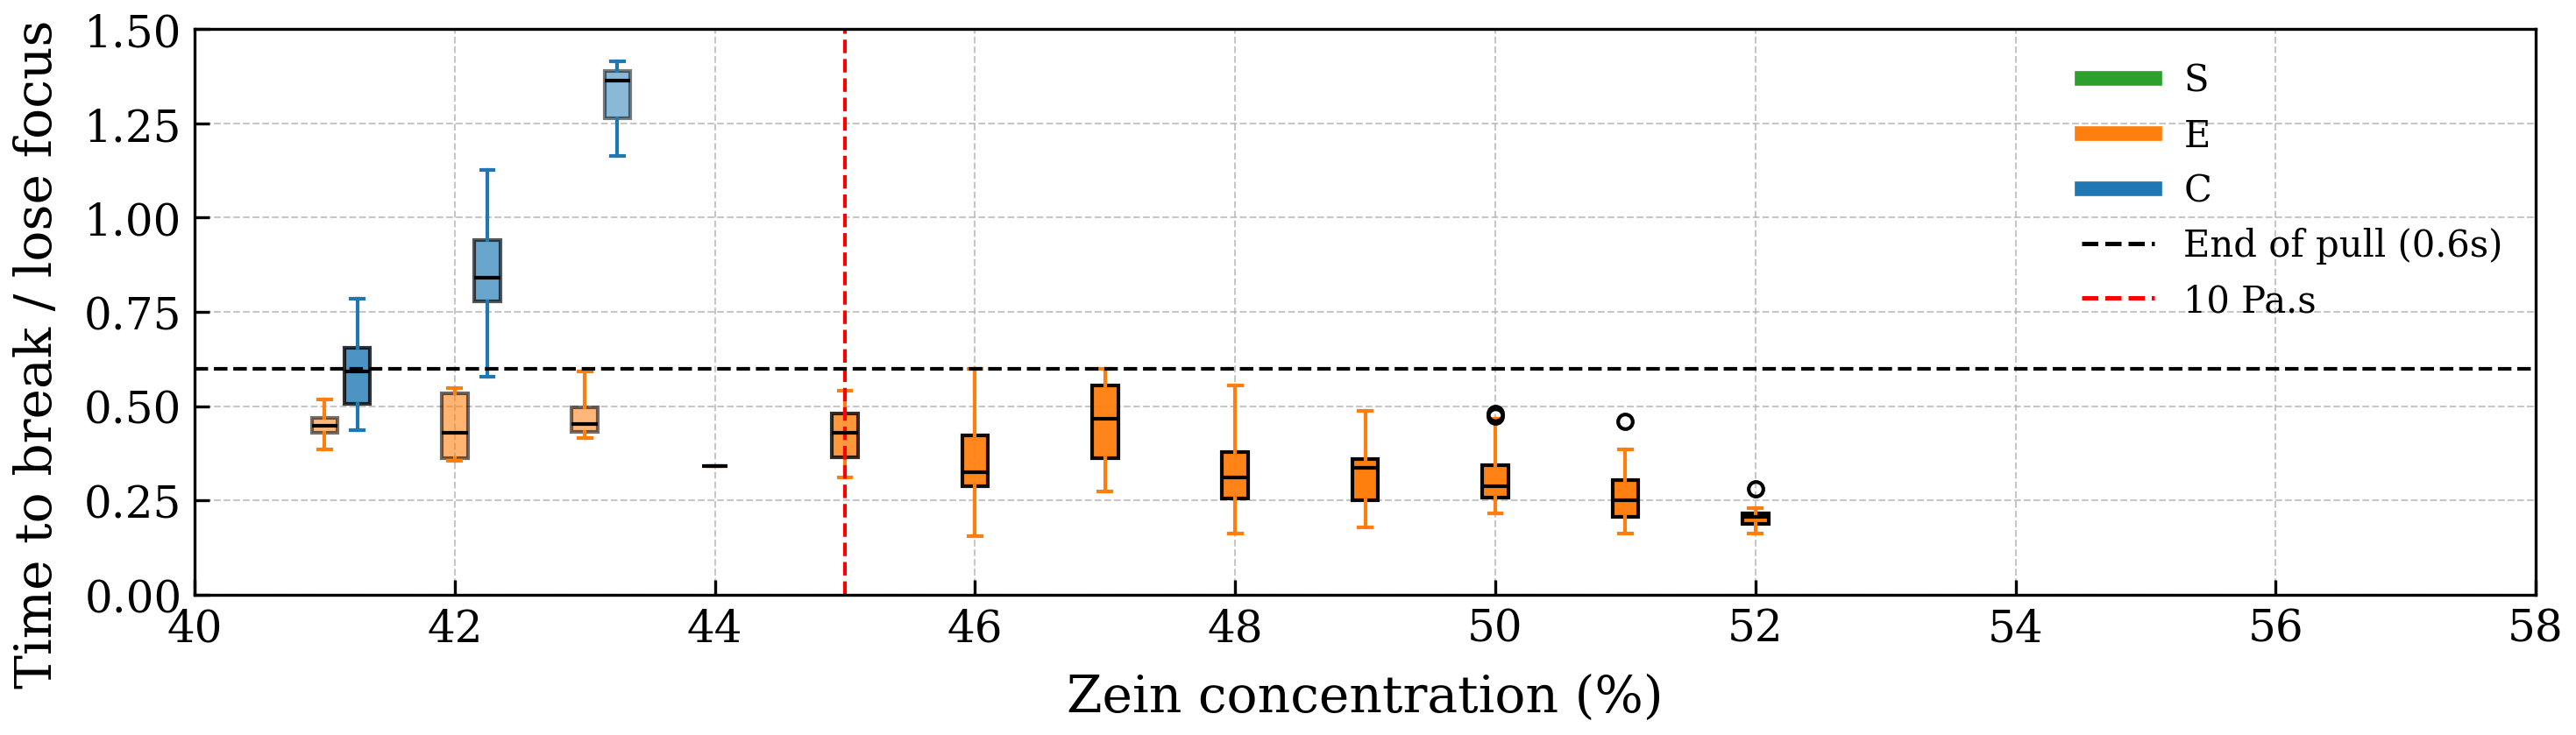
\includegraphics[width=0.7\textwidth]{figures/cone_analysis/time_by_etoh_90.png}
        \put(-150, 58){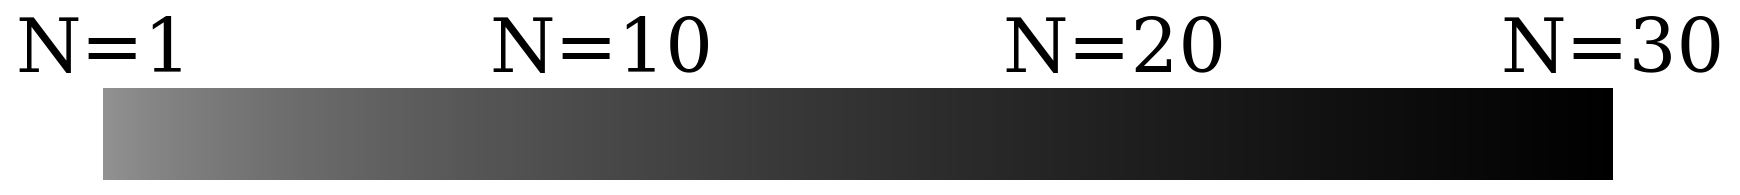
\includegraphics[width=0.25\textwidth]{figures/cone_analysis/shade_bar.png}}
	\caption{
		Box plots of time to break as a function of zein concentration for the 90\% ethanol condition.
		Box plots are grouped by failure mode: success (s, green), elastic failure (e, orange), and capillary failure (c, blue). 
		Medians are shown as solid black lines within each box. 
		Box transparency is scaled with the number of trials to indicate sample size as is indicated by the shading map.
		Outliers are shown as white dots.
		The horizontal dashed line indicates the time at which the pin stops moving.
	}
	\label{fig:time_by_etoh_90}
\end{figure}

\subsection{Is there a lower molecular weight limit below which skin formation does not stabilize a protein solution liquid bridge?}
So far we have shown that contact drawing of 22 kDa zein solutions in a volatile solvent (ethanol/water) is possible due to skin formation. To test the limit of this concept, we investigated contact drawing of water solutions containing cod collagen I peptides with a molecular weight of 2-5 kDa. The peptides were soluble in water up to 80\% by weight, reached a zero-shear viscosity of 160 Pa$\cdot$s at that concentration (figure \ref{fig:flow_sweep_example}) and could be drawn into 10 cm long fibers (figure \ref{fig:collagen_peptide}A) with a 95\% success rate at a draw velocity of 25 to 50 mm/s over distances ranging from 30 to 100 mm (N=20). A 4 to 10-fold decrease in molecular weight led to a 20-fold increase in the minimum viscosity required to draw fibers at a reasonable velocity. In comparison, the polymer reptation model mentioned above would predict a minimum draw velocity around 1 km/s which is completely unrealistic. Furthermore scanning electron microscopy pictures of the collagen peptide fibers hand drawn using a pin array \cite{yaghoobi_multifilament_2023} revealed a wrinkled surface consistent with the formation of a dried skin (figure \ref{fig:collagen_peptide}B).

\begin{figure}[htb]
	\centering
	% Taken form the ~/lab/cod_collagen/ repo
	% Frame 38 -> t = 0.00 s (fps = 135)
	% Frame 76 -> t = 0.28 s
	% Frame 330 -> t = 2.16 s (fps = 135)
	%\begin{overpic}[width=4.8cm, trim=0 0 0 0, clip]{figures/diameter_trace/cod_example.png}
	%	\put(2, 55){\tiny \color{black}(A)}

	%	\put(25, 52){\tiny \color{black}(1)}
	%	\put(21.5, 54){\color{black}$\star$}

	%	\put(65, 45){\tiny \color{black}(2)}
	%	\put(68, 40){\color{black}$\star$}

	%	\put(21, 16){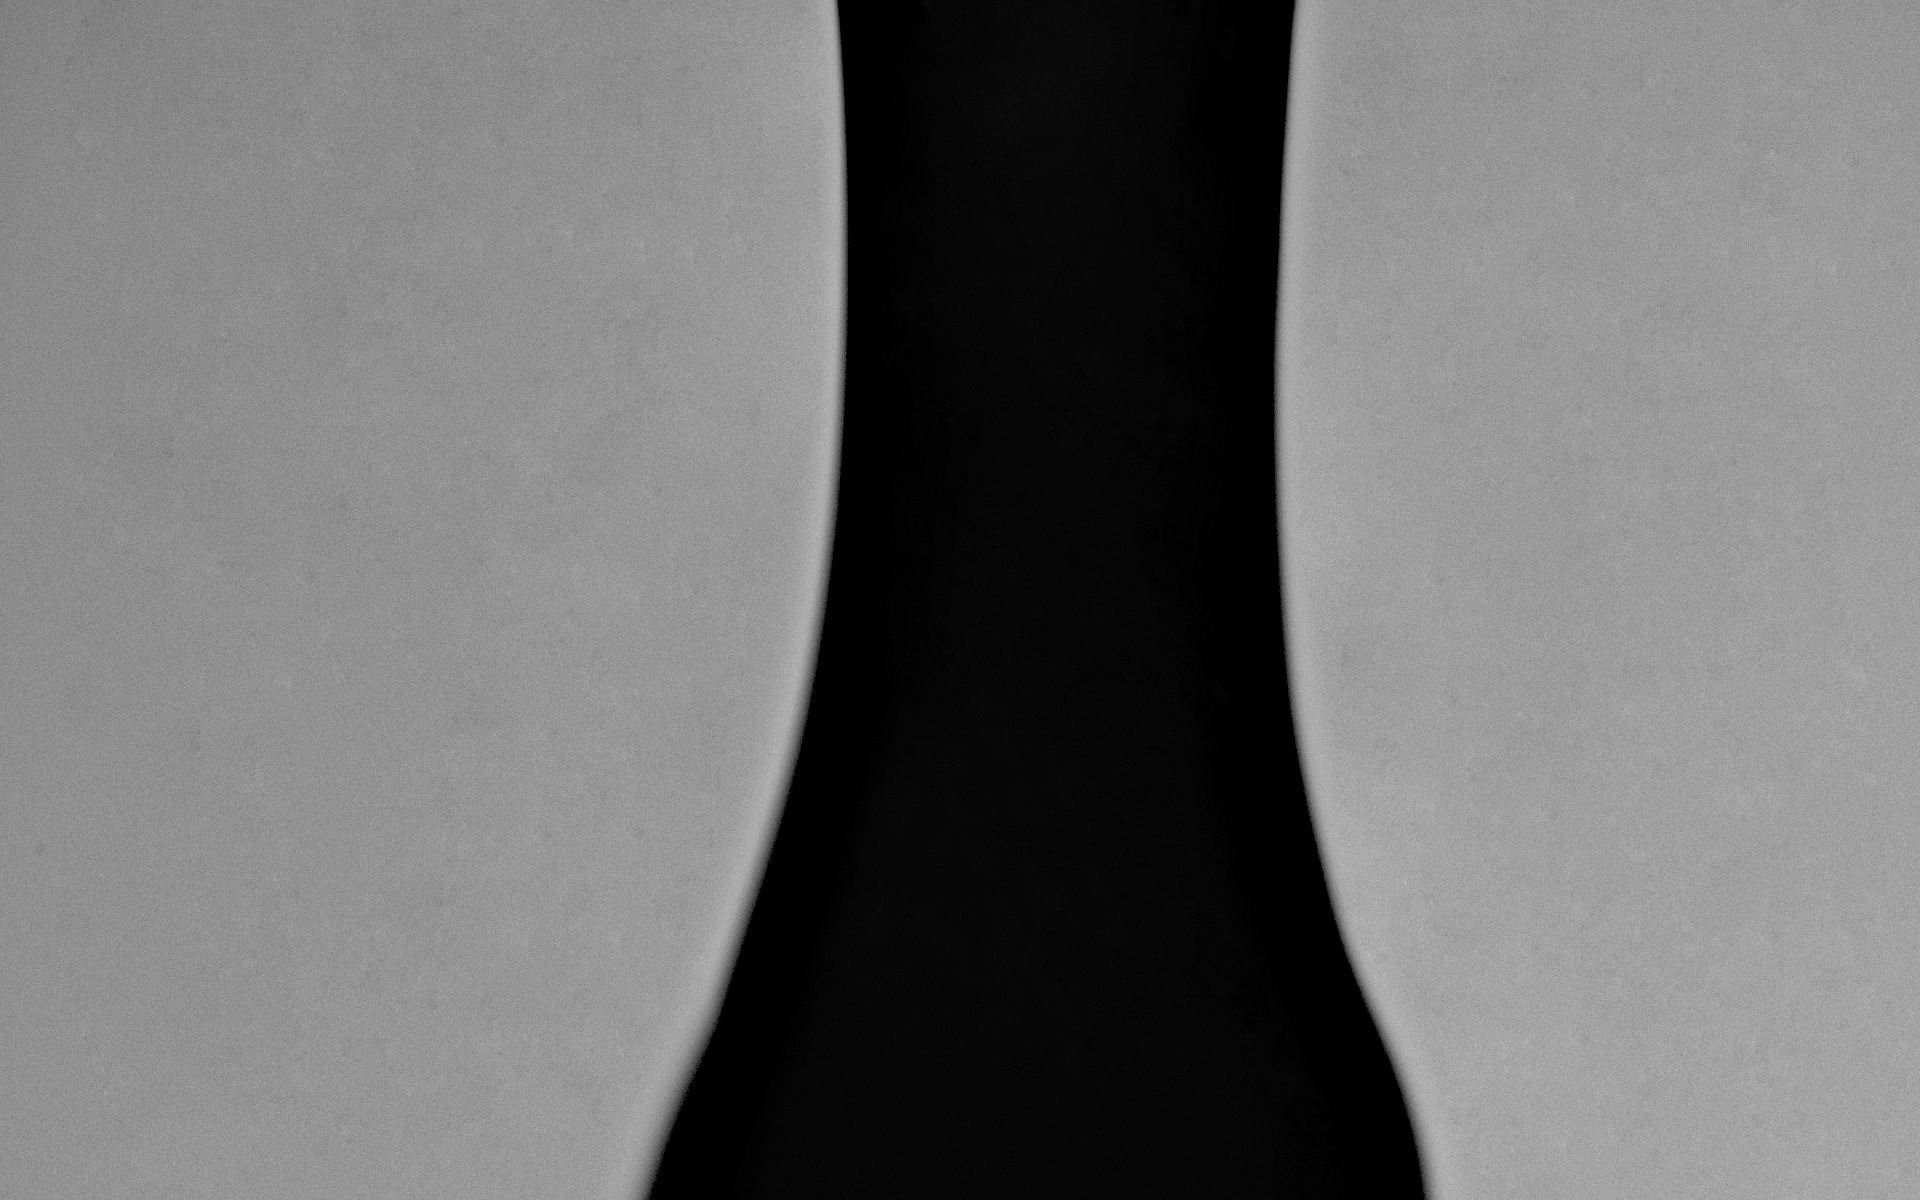
\includegraphics[width=1.1cm, trim=200 0 200 0, clip]{figures/cone_images/cod_tif/image_fps135_00076_edit.png}}
	%	\put(52, 16){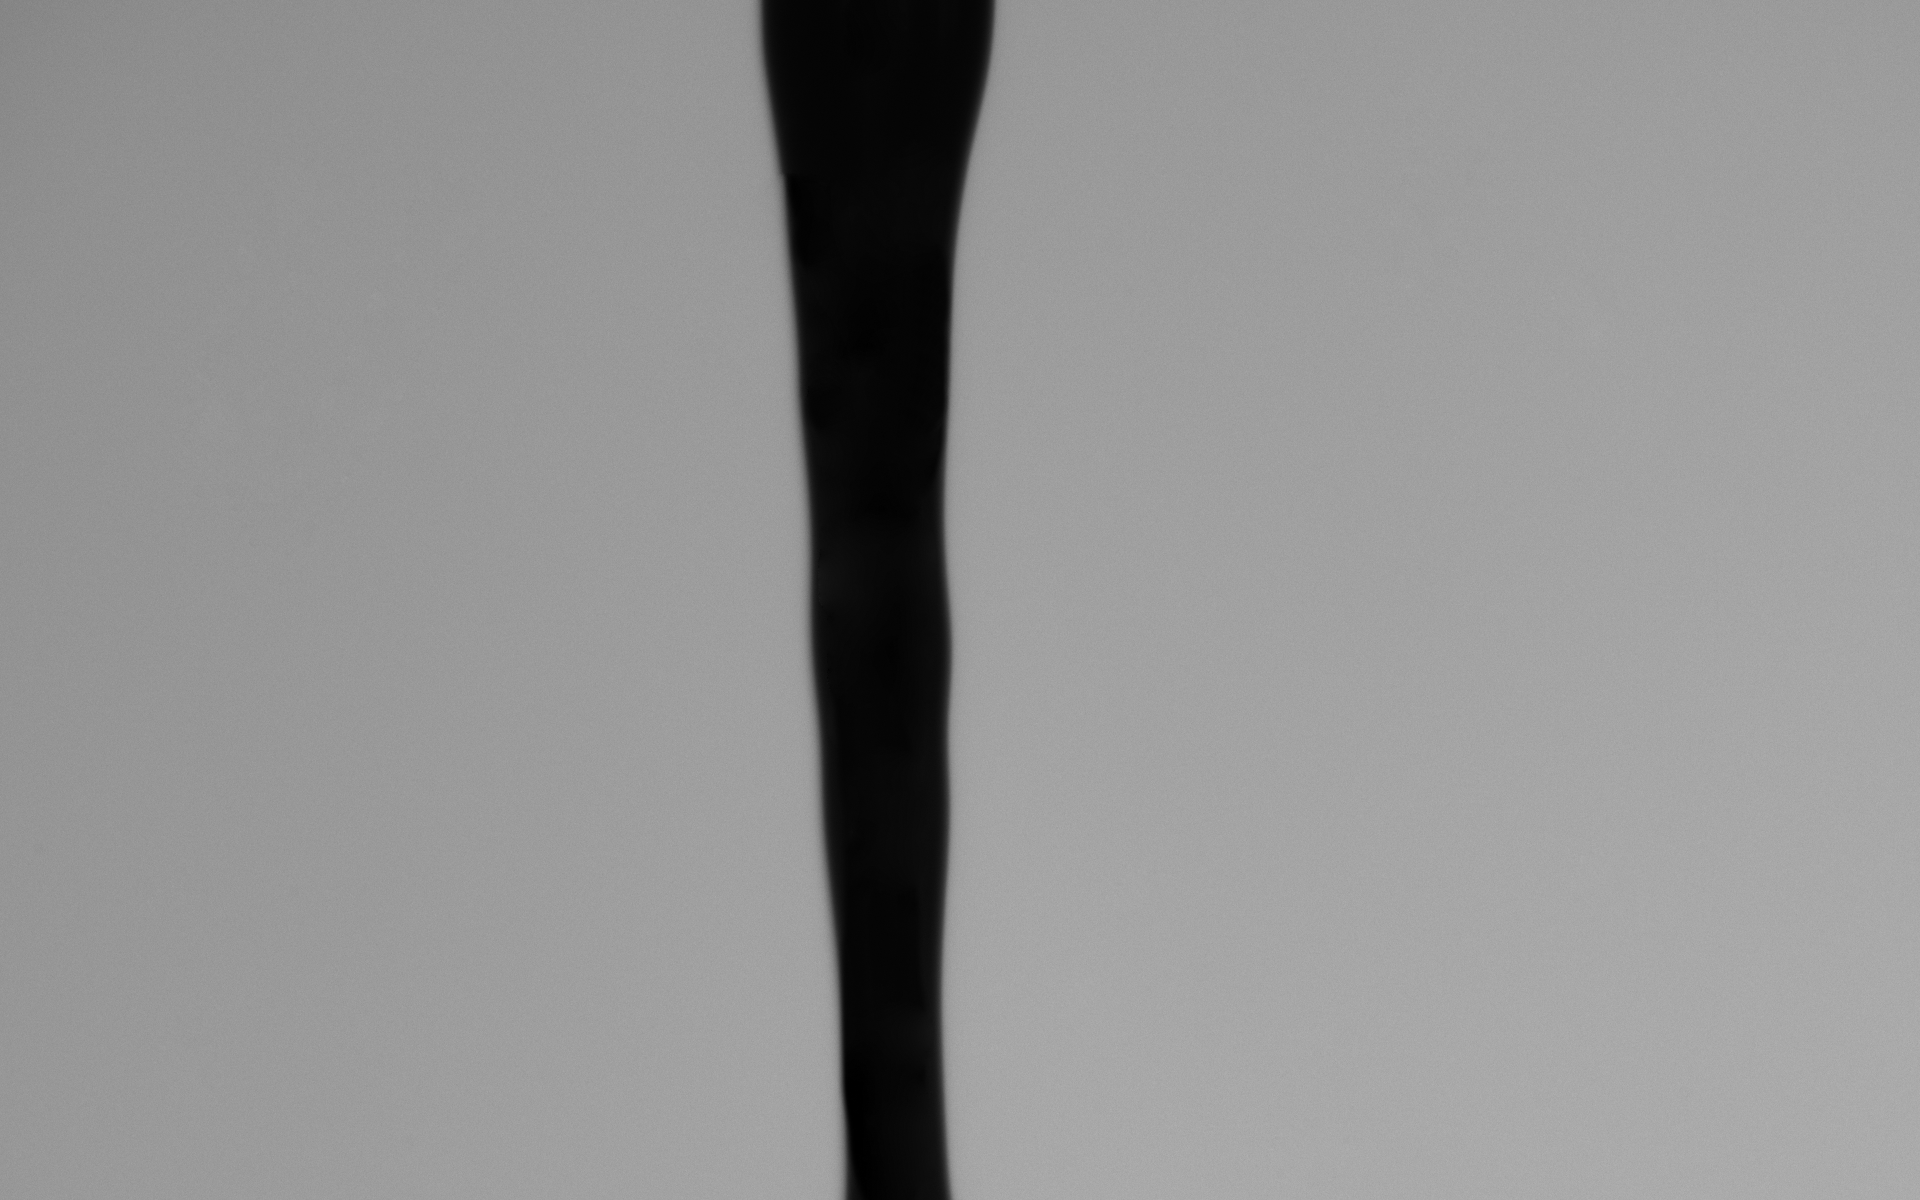
\includegraphics[width=1.1cm, trim=200 0 200 0, clip]{figures/cone_images/cod_tif/image_fps135_00330_edit.png}}
	%	\put(22, 30){\tiny 1}
	%	\put(53, 30){\tiny 2}
	%\end{overpic}
	%\raisebox{0.41cm}{
	%\begin{overpic}[width=3.0cm, trim=0 200 400 0, clip]{figures/sem/Cod_SEM.png}
	%	% White background
	%	\put(-1,75){\colorbox{white}{\tiny B}}
	%	\put(2, 11){\tiny \color{white}1$\mu$m}
	%	\put(5, 6){\color{white}\rule{7.9pt}{2pt}} % Calibrated!
	%\end{overpic}
	%}
    \centering
    \def\svgwidth{0.8\textwidth} % or 0.48\textwidth for half-width
    \import{figures/panels/}{cod_figure.pdf_tex}
	\caption{
		(A) Example of successfully drawn 80\% cod collagen I peptide fibers in water. 
		Labeled points (1) and (2) correspond to the cone images in panel (A).
		The solution is composed of 80\% cod collagen in water. 
		The solution is drawn with an acceleration of 1000 mm/s$^2$ until a maximum draw velocity of 25 mm/s is reached over a distance of 100 mm.
		(B) Scanning electron microscopy image of a dried cod collagen I peptide fiber showing a wrinkled surface consistent with skin formation.
		The solution is composed of 80\% cod collagen in water.
		The solution was drawn using a hand held pin array. 
	}
	\label{fig:collagen_peptide}
\end{figure}

\section{Conclusions}
We demonstrate that low molecular weight proteins (zein: 22kDa and cod collagen peptides: 2-5 kDa) are capable of forming fibers by contact drawing. Unlike entangled high molecular weight polymer solutions (70-500kDa), where fiber formation is governed by reptation time, protein solution liquid bridges can stabilize through the formation of a solid-like skin that resists capillary thinning. Our results indicate that this stabilization mechanism is concentration and solvent dependent, with a narrow viscosity window enabling fiber formation by minimizing capillary and elastic failures. High-speed imaging reveals that the timing of skin formation governs the thinning dynamics and determines failure modes. This work broadens the applicability of contact drawing to protein solutions and suggests that skin formation is a robust and tunable mechanism for fiber fabrication in lower molecular weight systems.

\bibliographystyle{jfm}
\bibliography{references}


\end{document}
